\documentclass[a4paper, 11pt, titlepage]{jsarticle}
\usepackage{graphicx}
\usepackage[dvipdfmx]{color}
\usepackage{amsmath}
\usepackage{listings}
\usepackage{url}

\title{知能情報実験 I\hspace{-1.2pt}I\hspace{-1.2pt}I グループ 1 \\ テーマ:株価予測}
\author{225752B PARK CHEOLHWAN \\ 225741G 清水 優馬 \\ 225745K 大石根 竜馬 \\ 225754J 當山 一朗}
\date{\today}

\begin{document}
\maketitle
\tableofcontents
\clearpage

\section{はじめに}
\subsection{実験の目的と達成目標}
\indent 知能情報実験 I\hspace{-1.2pt}I\hspace{-1.2pt}Iは、情報工学分野のより専門的な知識を理解・習得することを目的として、半年間でシステムの開発やデータ解析等に取り組む実施される。その中の一つデータマイニング班においては機械学習外観ならびにその応用を通し、対象問題への理解、特徴量抽出等の前処理、バージョン管理やデバッグ・テスト等を含む仕様が定まっていない状況下における開発方法、コード解説や実験再現のためのドキュメント作成等の習得を目指す。
\subsection{テーマ: 株価予測とは}
\indent 本グループでは、個人投資家の株の投資における将来の株価を予測することを対象問題として設定した。\\
\indent 株価予測とは、市場に出回っている株価の推移を予測することであり、テクニカル分析やファンダメンタルズ分析を使って予測することが一般的である。今回の実験では、数値データとして扱うことができるデータの多いテクニカル分析を用いて株価予測を実施する。テクニカル分析とは、参考文献 \cite{tech}によると、 移動平均線、株価チャートなど、株価データの「型」(=パターン)を基礎に、相場の先行きを予測することである。また、株価の変動は、様々な要因によって引き起こされる。例えば、企業の業績や経済指標、政治情勢、自然災害などが挙げられる。これらの要因を分析し、株価の変動を予測することで、投資家はリスクを最小限に抑えながら、収益を最大化することができる。\\

\section{実験方法}
実験方法としては、下記のような手順で進める予定で進むことにした。
\begin{itemize}
  \item 実験目的:実験を進む前に、実験で進むテーマを明確にし、目的を設定し、テーマとしては、株価予測を選定した。
  \item データセット構築:株価データを取得し、テクニカル分析を行うためのデータセットをYfinance APIを用いて構築し、実験の対象としては、時事的な要因が少ない株価である1321.T(日経225)を選定した。
  \item モデル選定:株価予測に有効なモデルを探すために、資料などを参考にした結果、LSTM(Long Short-Term Memory)モデルを選定した。
  \item パラメータ調整:LSTMモデルのパフォーマンスを最適化するために、いくつかのパラメータを調整した。パラメータ調整としては、エポック数、バッチサイズ、LSTMユニット数、Dense層、学習率、データの正規化を調整した。
  \item 結果:実験結果をまとめ、考察を行い、意図していた実験計画との違いを検討し、まとめを行った。
\end{itemize}
\subsection{実験目的}
\indent 本グループでは、株価予測モデルの有効性を検証することを目的としている。具体的には、テクニカル分析を用いた移動平均線や株価チャートのパターン認識を通じて、株価の変動をどの程度正確に予測できるかを明らかにする予定である。また、異なる分析手法やパラメータの組み合わせが予測精度に与える影響を確認し、最適な予測モデルを特定することを目指している。

\subsection{データセット構築}
\indent yfinance APIを用いて、株価データを取得する。取得したデータは、Open, High, Low, Close, Volume, Dividends, Stock Splitsの7つのカラムからなる(Dateは除く)。また、取得したデータを元に、直近3年間の株価データを取得し、テクニカル分析を行うことができるデータセットを構築する。\\
\indent yfinance APIのURLは、参考文献\cite{yfin}である。

\subsection{モデル選定}
\indent 本実験では、株価予測において有効であると判断したLSTM(Long Short-Term Memory)モデルを用いる。LSTMは、リカレントニューラルネットワーク(RNN)の一種であり、特に時系列データの予測に優れた性能を発揮する。LSTMモデルは、過去のデータの長期依存性を捉えることができるため、株価のように時間に依存するデータに対して有効である。また、LSTMは従来のRNNに比べて勾配消失問題を解決する設計がなされており、長期間の依存関係を効果的に学習できるため、株価の変動パターンを正確に予測することが期待できる。このため、本実験ではLSTMモデルを選定した。
\subsection{パラメータ調整}
\indent 本実験では、LSTMモデルのパフォーマンスを最適化するために、いくつかのパラメータを調整しました。また、下記は主要なパラメータとその調整過程を示している。また、下記は、パラメータを調整する際のログを示している。
\lstinputlisting[language=, frame=single, breaklines=true, caption={バッチサイズが1の場合}, label=one]{./parameter/one.txt}
\lstinputlisting[language=, frame=single, breaklines=true, caption={バッチサイズが16の場合}, label=two]{./parameter/two.txt}
\lstinputlisting[language=, frame=single, breaklines=true, caption={バッチサイズが32の場合}, label=three]{./parameter/three.txt}
\lstinputlisting[language=, frame=single, breaklines=true, caption={バッチサイズが2048の場合}, label=four]{./parameter/four.txt}

\indent 上記のListing \ref{one}、Listing \ref{two}、Listing \ref{three}、Listing \ref{four}を通じて、エポック数は20~30が最適であることがわかった。また、バッチサイズは16が最適であることがわかった。よって、下記のようにパラメータを設定した。
\paragraph{エポック数}
\indent Listing \ref{}
\indent モデルの訓練において、エポック数は重要なパラメータである。本実験では、エポック数を20に設定した。将来的には、エポック数を増やすことでモデルの収束状況や予測精度が向上する可能性があるため、さらに検討する予定である。

\paragraph{バッチサイズ}
\indent バッチサイズもモデルの性能に影響を与える重要なパラメータである。本実験では、バッチサイズを16に設定した。この設定は計算効率と予測精度のバランスを考慮したものである。将来的には異なるバッチサイズを試し、最適なバッチサイズを特定することを計画する予定である。

\paragraph{LSTMユニット数}
\indent LSTM層のユニット数は、モデルのキャパシティに直接影響する。本実験では、2つのLSTM層を使用し、各層のユニット数を128および64に設定した。将来的には、ユニット数を増やしてモデルの予測性能がどのように変化するかを評価し、最適なユニット数を決定する予定である。

\paragraph{Dense層}
\indent Dense層は、LSTM層の出力を線形変換し、最終的な予測値を生成する。本実験では、LSTM層の後に2つのDense層を追加し、最終的な出力層のユニット数を1に設定した。これにより、時系列データの特徴を捉えた後、適切な予測値を生成することが可能となった。

\paragraph{学習率}
\indent 最適化アルゴリズムの学習率は、モデルの収束速度と安定性に影響を与える。本実験では、デフォルトの学習率(0.001)を使用した。将来的には、異なる学習率(例えば0.01や0.0001)を試し、モデルの収束速度と安定性を最適化することを検討する予定である。

\paragraph{データの正規化}
\indent データの正規化は、モデルの収束速度と予測精度に大きな影響を与える。本実験では、MinMaxScalerを使用してデータを0から1の範囲にスケーリングした。将来的には、標準スケーリングやロバストスケーリングなどの他のスケーリング手法も試して、モデルの性能向上を図る予定である。

\section{実験結果}
\begin{figure}[htbp]
  \centering
  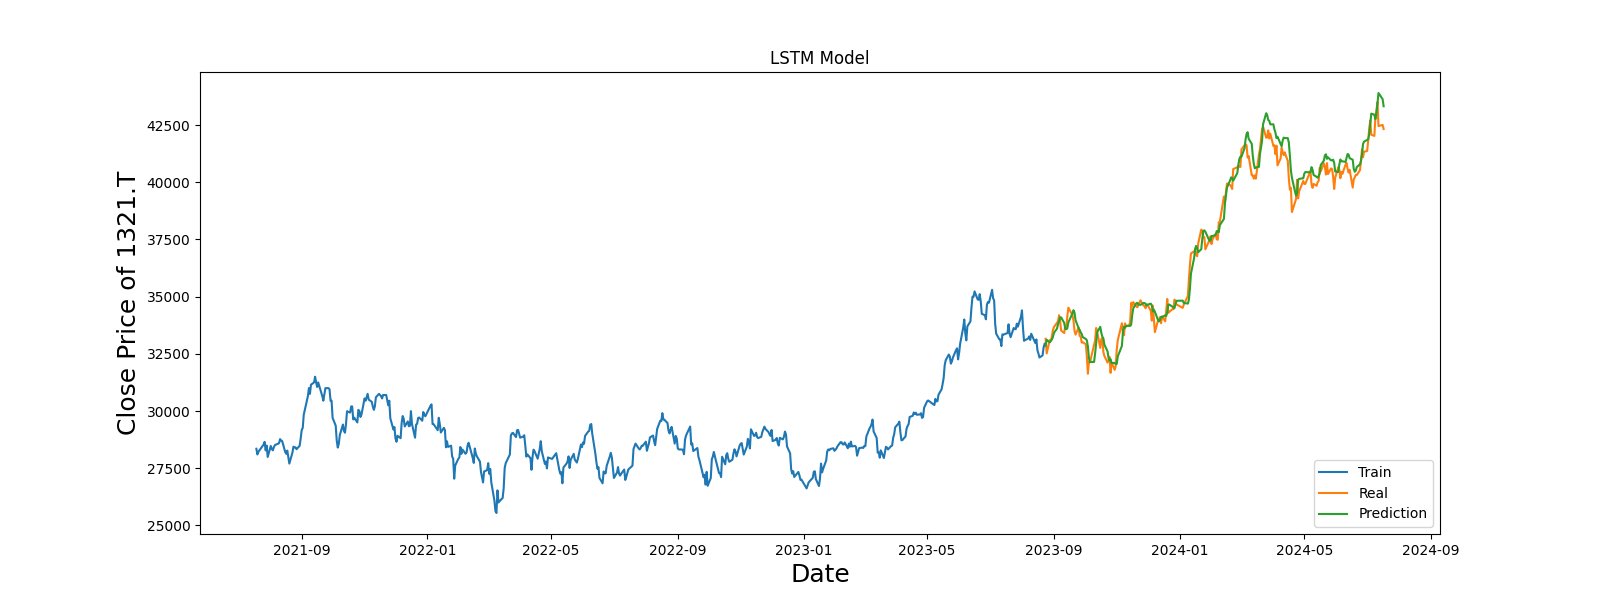
\includegraphics[width=120mm]{./exericise/image/lstm_model.png}
  \caption{exericiseのtest\_two.pyの実行結果}
  \label{twopython}
\end{figure}

\section{考察}
未着手

\section{意図していた実験計画との違い}
未着手

\section{まとめ}
未着手

\begin{thebibliography}{99}
  \bibitem{tech} 野村證券株式会社、証券用語解説集、テクニカル分析、\url{https://www.nomura.co.jp/terms/japan/te/tec_analysis.html}。
  \bibitem{yfin} yfinance API、\url{https://pypi.org/project/yfinance/}。
  \bibitem{Sequential model} Kerasライブラリ、Sequential model、\url{https://keras.io/guides/sequential_model/}。
  \bibitem{Dense layer} Kerasライブラリ、Dense layer、\url{https://keras.io/api/layers/core_layers/dense/}。
  \bibitem{LSTM layer} Kerasライブラリ、LSTM layer、\url{https://keras.io/api/layers/recurrent_layers/lstm/}。
  
\end{thebibliography}
\end{document}